\documentclass{report}
\usepackage[utf8]{inputenc}
\usepackage{graphicx}
\usepackage[portuguese]{babel}
\usepackage[margin=2cm]{geometry}

\title{ 
\includegraphics[scale=0.3]{logo.png} \\ \textbf{Off Constructions - O uso de bases de dados aplicadas à construção civil}}

\author{Bases de Dados \\ Mestrado Integrado em Engenharia Informática e Computação \\ \\ G504 \\ Afonso Carvalho up201807481@fe.up.pt \\ Tiago Rodrigues up201907021@fe.up.pt \\ Tomás Fidalgo up201906743@fe.up.pt}

\graphicspath{{./images/}}

\begin{document}
	\maketitle
	
	\tableofcontents
	
	\chapter{Introdução}
		\paragraph{}A OFF Constructions, uma empresa de construção sediada no Porto, pretende
		armazenar informação relativa ao seu funcionamento, com o propósito de tornar o seu
		negócio mais eficiente. Deste modo, foi-lhes sugerida a seguinte base de dados:
		
		\section{Requisitos do cliente}
		
			\paragraph{•}Do cliente é guardada informação relativa à sua identificação, por
			motivos de faturação. Assim, é necessário guardar o nome, o contacto telefónico, a
			morada e o seu NIF. Quando o cliente requisita uma obra, é primeiro criado um
			projeto, que contém detalhes relativos ao orçamento acordado e ao prazo de
			finalização. Um cliente pode requisitar mais do que uma obra, no entanto, cada
			obra terá apenas um cliente, seja ele particular ou outra empresa.
		
		\section{Requisitos da obra}
		
			\paragraph{•}De cada obra interessa saber a sua localização (rua, Nº de porta,
			código postal e cidade), a data de início das construções, o custo real (que tanto
			pode ser superior como inferior ao orçamento), a área de terreno envolvida assim
			como a área interior projetada. Por fim, é necessário saber, a um dado instante, o
			estado da obra.
			
		\section{Requisitos de material}
			
			\paragraph{•}Cada obra tem, de antemão, uma certa quantidade de material
			alocado, do qual se pretende saber a quantidade disponível e o custo. Cada
			material diferente possui um código interno, assim como uma designação pela qual
			é conhecido. Este material é guardado num dos estaleiros da empresa (a OFF
			Constructions prefere guardar todo o material igual no mesmo estaleiro), dos
			quais é importante saber a localização (com os mesmos requisitos da obra) e
			capacidade máxima.
			
		\section{Requisitos de veículos}
		
			\paragraph{•}Para além do material, a empresa possui uma frota de veículos,
			tanto de transporte de empregados como de materiais, assim como todos os tipos
			de maquinaria pesada usada nas diferentes obras. De cada veículo, a empresa
			gostaria de registar a matrícula, a categoria (segundo o código da estrada), as
			despesas associadas, o consumo médio do veículo bem como a data de inspeção de
			cada um.
			
		\section{Requisitos dos empregados}
		
			\paragraph{•}Por último, a OFF gostaria de registar todos os seus empregados no
			sistema. Todos os empregados têm o seu nome, NIF, contacto e salário registados,
			assim como a sua habilitação escolar. Dos empregados que estão nas obras,
			interessa saber a sua especialidade (carpinteiro, eletricista, etc.) e o cargo
			que possui na obra. Quanto aos empregados que estão no escritório, é necessário
			guardar a sua estação de trabalho e a sua especialização (decorador,
			contabilista, arquiteto, engenheiro, entre outras). Outro tipo de empregados que
			a OFF contrata são maquinistas, cujo trabalho é operar e manobrar os vários
			veículos usados nas obras. Posto isto, de cada um deles é necessário saber as
			categorias (segundo o código da estrada) que estão habilitados a conduzir.
				
			\begin{figure}[hb!]
				\centering
				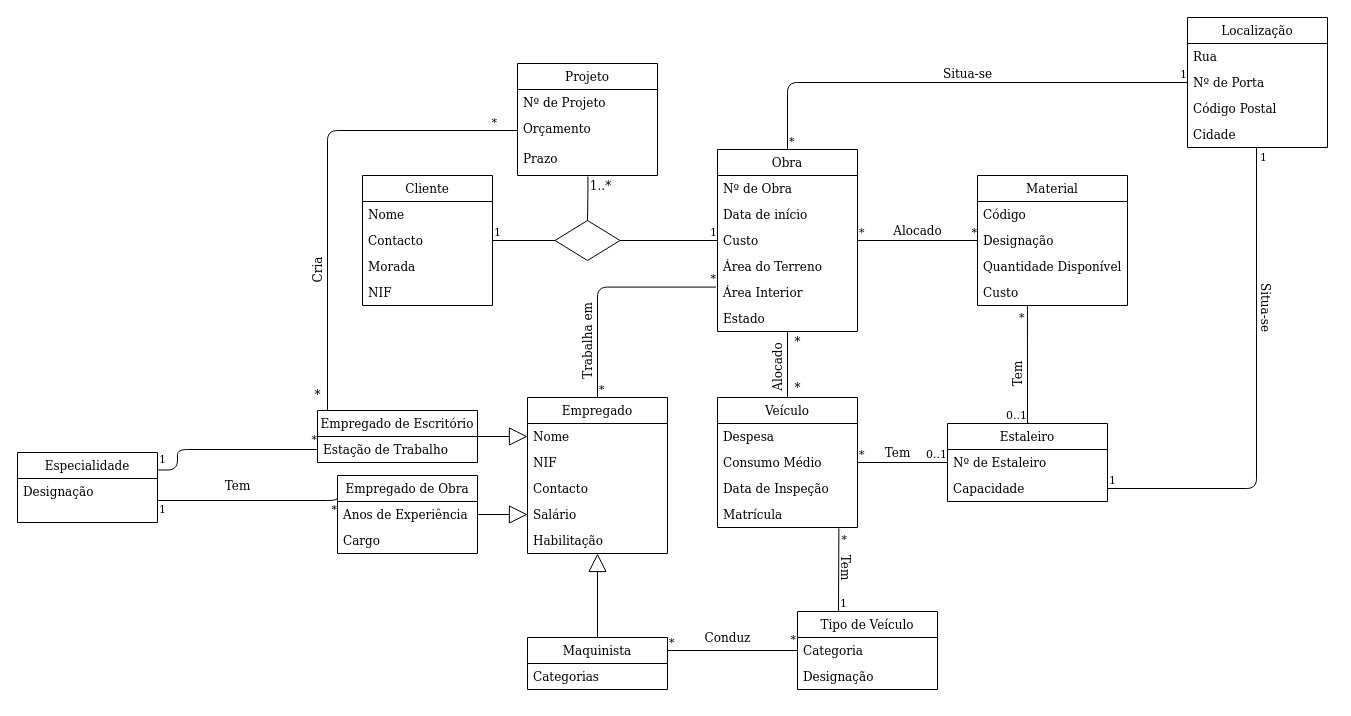
\includegraphics[scale=0.45, angle=-90]{UML-Original.png}
				\caption{Diagrama UML original correspondente aos requisitos dados}
			\end{figure}
		
		\section{Novos requisitos}
			
			\paragraph{•}Após falar com o docente, foram propostas algumas ligeiras
			alterações ao modelo apresentado, as quais podem ser vistas no seguinte diagrama
			UML.
			
			\begin{figure}[hb!]
				\centering
				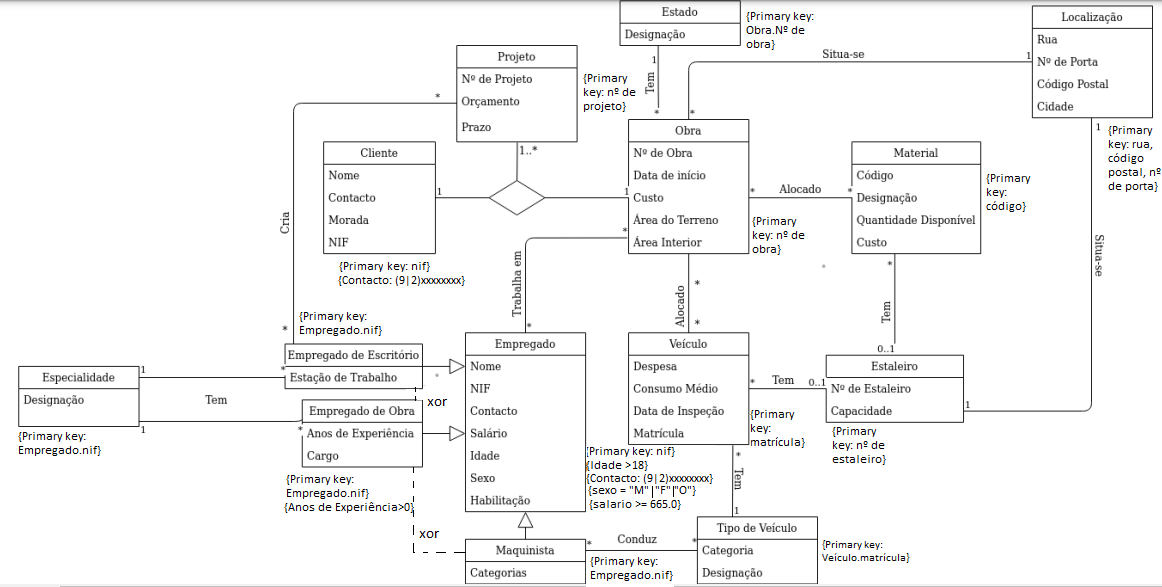
\includegraphics[scale=0.44, angle=-90]{UML-Revisto.png}
				\caption{Diagrama UML revisto correspondente aos novos requisitos}
			\end{figure}
	\chapter{Esquema Relacional}
	
		\paragraph{•}O diagrama UML revisto poderá ser decomposto no seguinte esquema
		relacional, e são possíveis obter as seguintes tabelas.
		
		\begin{itemize}
			\item $Cliente(Nome,\ Morada,\ Contacto,\ NIF)$
			\item $Projeto(N\ de\ Projeto,\ Orcamento,\ Prazo)$
			\item $Obra(N\ de\ Obra,\ Data\ de\ Inicio,\ Custo,\ Area\ do\ Terreno,\ Area\
			Interior,\ Estado \rightarrow Estado,\ Rua \rightarrow Localizacao.Rua,\ N\ de\ 
			Porta \rightarrow Localizacao.N\ de\ Porta,\ Codigo\ Postal \rightarrow
			Localizacao.Codigo\ Postal)$
			\item $Estado(Designacao)$
			\item $Material(Codigo,\ Designacao,\ Quantidade\ Disponivel,\ Custo,\ Guardado
			\rightarrow Estaleiro)$
			\item $Localizacao(Rua,\ N\ de\ Porta,\ Codigo\ Postal,\ Cidade)$
			\item $Estaleiro(N\ de\ Estaleiro,\ Capacidade,\ Rua \rightarrow Localizacao.Rua,\
			N\ de\ Porta \rightarrow Localizacao.N\ de\ Porta,\ Codigo\ Postal \rightarrow
			Localizacao.Codigo\ Postal)$
			\item $Veiculo(Matricula,\ Consumo\ Medio,\ Data\ de\ Inspecao,\ Despesa,\ Tipo 
			\rightarrow TipoDeVeiculo,\ Guardado \rightarrow Estaleiro)$
			\item $TipoDeVeiculo(Categoria,\ Designacao)$
			\item $Especialidade(Designacao)$
			\item $Empregado(Nome,\ NIF,\  Contacto,\ Salario,\ Habilitacao,\ Idade,\ Sexo)$
			\item $EmpregadoDeEscritorio(NIF \rightarrow Empregado,\ Estacao\ de\ Trabalho,\
			Especialidade \rightarrow Especialidade)$
			\item $EmpregadoDeObra(NIF \rightarrow Empregado,\ Anos\ de\ Experiencia,\ Cargo,\
			Especialidade \rightarrow Especialidade)$
			\item $Maquinista(NIF \rightarrow Empregado,\ Categorias)$
			\item $Cria(NIF \rightarrow EmpregadoDeEscritorio,\ N\ de\ Projeto \rightarrow
			Projeto)$
			\item $MaterialAlocado(Codigo\rightarrow Material,\ N\ de\ Obra \rightarrow Obra)$
			\item $VeiculoAlocado(Matricula \rightarrow Veiculo,\ N\ de\ Obra \rightarrow
			Obra)$
			\item $TrabalhaEm(NIF \rightarrow Empregado,\ N\ de\ Obra \rightarrow Obra)$
			\item $Conduz(NIF \rightarrow Maquinista,\ Designacao \rightarrow TipoDeVeiculo)$
			\item $ClienteObraProjeto(Cliente \rightarrow Cliente,\ Obra \rightarrow Obra,\
			Projeto  \rightarrow Projeto)$
		\end{itemize}
	
	\chapter{Dependências Funcionais}
	
		\paragraph{}Fazendo uma pequena análise das dependências funcionais é possível
		determinar as seguinte.
		
		\begin{itemize}
			\item Na relação cliente:
			\begin{itemize}
				\item $NIF \rightarrow Nome,\  Morada,\ Contacto$
				\item $Contacto \rightarrow Nome$
			\end{itemize}
			
			Uma vez que a DF Contacto $\rightarrow$ Nome existe, e Contacto não é uma
			chave, a relação apresenta uma violação à BCNF. Para além disto, como Nome também
			não é primo, a relação também não se encontra na 3FN.
			
			\item Na relação Projeto:
			\begin{itemize}
				\item $N\ de\ Projeto \rightarrow Orcamento,\ Prazo$
			\end{itemize}
			
			Como apenas temos uma DF e o lado esquerdo é uma chave, esta relação encontra-se
			na BCNF e, portanto, na 3FN também.
			
			\item Na relação Obra:
			\begin{itemize}
				\item $N\ de\ Obra \rightarrow Data\ de\ Inicio,\ Custo,\ Area\ do\ Terreno,
				Area\ Interior,\ Estado,\ Rua,\ N\ de\ Porta,\ Codigo\ Postal$
				\item $Rua,\ Codigo\ Postal,\ N\ de\ Porta,\ Data\ de\ Inicio \rightarrow
				 Custo,\ Estado,\ Area\ do\ Terreno,\ Area\ Interior$
			\end{itemize}
			
			O lado direito da segunda DF apresentada não contém apenas atributos primos, por 
			exemplo, o custo. O custo nunca poderia ser parte de uma chave, pois não permite 
			identificar uma obra nem na mesma localização (é possível realizar duas obras no 
			mesmo sítio, por exemplo, uma expansão, e terem exatamente o mesmo custo), nem em 
			sítios separados (várias obras a custarem o mesmo). Assim sendo, a relação não 
			está na 3FN e portanto também não está na BCNF.
			
			\item Na relação Estado:
			\\ \\
			Uma vez que a relação Estado apenas apresenta um elemento e não existem 
			dependências funcionais, obrigatoriamente está contida na BCNF e também na 3FN.
			
			\item Na relação Material:
			\begin{itemize}
				\item $Codigo \rightarrow Designacao,\ Quantidade\ Disponivel,\ Custo,\ 
				Guardado$
				\item $Designacao \rightarrow Quantidade\ Disponivel,\ Custo$
				\item $Designacao,\ Estaleiro \rightarrow Codigo$
			\end{itemize}
			
			Uma vez que a segunda DF não tem apenas atributos primos do lado direito 
			(Quantidade Disponível e Custo não fazem parte de nenhuma chave), então a relação 
			não está na 3FN nem na BCNF.
			
			\item Na relação Localização:
			\begin{itemize}
				\item $Codigo Postal \rightarrow Cidade$
				\item $Cidade, Rua \rightarrow Codigo Postal$
			\end{itemize}
			
			A relação encontra-se na 3FN, porque Código Postal é uma chave, e portanto também 
			é um atributo primo. No entanto, como Cidade e Rua não podem compor uma chave, 
			esta relação não se encontra na BCNF.
			
			\newpage
			
			\item Na relação Estaleiro:
			\begin{itemize}
				\item $Rua,\ Codigo\ Postal, N\ de\ Porta \rightarrow N\ de\ Estaleiro$
				\item $N\ de\ Estaleiro \rightarrow Rua,\ Codigo\ Postal, N\ de\ Porta,\ 
				Capacidade.$
			\end{itemize}
			
			Como ambas as DF têm chaves nos lados esquerdos (visto que cada localização apenas 
			pode ter um estaleiro, também seria uma chave), então esta relação encontra-se na 
			BCNF.
			
			\item Na relação Veículo:
			\begin{itemize}
				\item $Matricula \rightarrow Consumo\ Medio,\ Data\ de\ Inspecao,\ Despesa,\ 
				Tipo, Guardado$
			\end{itemize}
			
			Uma vez que apenas a matrícula consegue identificar outras características do 
			veículo, e é a chave da relação, então Veículo encontra-se na BCNF.
			
			\item Na relação TipoDeVeículo:
			\begin{itemize}
				\item $Designacao \rightarrow Categoria$
			\end{itemize}

			Como apenas temos uma DF, e Designação é chave, TipoDeVeículo também pertence à 
			BCNF.
			
			\item Na relação Especialidade:
			\\ \\
			Visto que a relação é composta apenas por um elemento, não existem DF’s e a
			relação pertence obrigatoriamente à BCNF.
			
			\item Na relação Empregado:
			\begin{itemize}
				\item $NIF \rightarrow Nome,\ Contacto,\ Salario,\ Habilitacao,\ Idade,\ Sexo$
				\item $Contacto,\ Nome \rightarrow NIF,\ Salario,\ Habilitacao,\ Idade,\ Sexo$
			\end{itemize}
			
			A relação Empregado encontra-se na BCNF, porque todos os lados esquerdos das DF 
			são chaves da relação (Contacto e Nome identificam o NIF, que identifica as 
			restantes). Assim sendo, para além de estar na BCNF, também está na 3FN.
			
			\item Na relação EmpregadoDeEscritório:
			\begin{itemize}
				\item $NIF \rightarrow Estacao\ de\ trabalho,\ Especialidade$
				\item $Especialidade \rightarrow Estacao de trabalho$
			\end{itemize}
			
			Visto que a Estação de trabalho não é um atributo primo, e a Especialidade não é 
			uma chave, a relação não pode pertencer à 3FN, e por consequência nem à BCNF.
			
			\item Na relação EmpregadoDeObra:
			\begin{itemize}
				\item $NIF \rightarrow Anos\ de\ Experiencia,\ Cargo,\ Especialidade$
				\item $Anos\ de\ Experiencia \rightarrow Cargo$
			\end{itemize}
			
			Nesta relação, podemos ver que na segunda DF, nem o elemento da esquerda é chave, 
			nem o da direita é primo, logo, a relação não pertence a 3FN nem à BCNF.
			
			\item Na relação Maquinista:
			\begin{itemize}
				\item $NIF \rightarrow Categorias$
			\end{itemize}
			
			Como só existe uma DF possível, e o lado esquerdo é a chave da relação, então 
			Maquinista está na BCNF.
			
			\item Na relação Cria:
			\\ \\
			Dado que a relação é apenas composta por elementos que pertencem  à chave, não 
			existem DF’s e a relação está portanto na BCNF.
			
			\item Na relação MaterialAlocado:
			\\ \\
			A relação MaterialAlocado também não apresenta DF’s, pois todos os elementos são 
			parte da chave. Deste modo, encontra-se na BCNF.
			
			\item Na relação VeículoAlocado:
			\\ \\
			Aqui sucede-se o mesmo que em MaterialAlocado, e por todos os elementos serem 
			chaves, a relação está na BCNF e na 3FN.
			
			\item Na relação TrabalhaEm:
			\\ \\
			Mais uma vez, como todos os elementos são chaves, a relação está na BCNF e na 3FN, 
			devido à falta de DF’s.
			
			\item Na relação Conduz:
			\\ \\
			Visto que a relação apenas contém elementos que fazem parte da chave, não existem 
			DF’s e a relação encontra-se na BCNF e 3FN.
			
			\item Na relação ClienteObraProjeto:
			\begin{itemize}
				\item $Projeto \rightarrow Obra,\ Cliente$
				\item $Obra \rightarrow Cliente$
			\end{itemize}
			
			Como a Obra não é uma chave, e Cliente não é um atributo primo, a relação 
			ClienteObraProjeto não satisfaz os requisitos para pertencer à 3FN, e, por 
			consequência, também não pode estar na BCNF.
		\end{itemize}
		
	\chapter{Restrições Associadas}
		
		\paragraph{}Para assegurar consistência entre os dados, as seguintes relações foram
		impostas na base de dados.
		
		\begin{itemize}
			\item Na relação Cliente:
			\begin{itemize}
				\item Não podem haver elementos NULL: Restrições NOT NULL.
				\item NIF terá que ser válido e único. Por questões de simplicidade, verifica-
				se apenas se está no intervalo correto, sem assegurar a validez dos dígitos: 
				Restrições CHECK e PRIMARY KEY.
				\item Contacto tem de corresponder a um número de telefone para uso pessoal, 
				que em Portugal começam pelo indicativo 9, se forem telemóveis, ou 2, se forem 
				telefones fixos: Restrição CHECK.
			\end{itemize}
			\item Na relação Projeto:
			\begin{itemize}
				\item Não podem existir elementos NULL: Restrições NOT NULL.
				\item Elementos têm de ser positivos: Restrições CHECK.
				\item Nº de projeto tem de ser único: Restrição PRIMARY KEY.
			\end{itemize}
			\item Na relação Obra:
			\begin{itemize}
				\item Com a exceção de data de início e áreas interiores e exteriores nenhum 
				campo poderá ser NULL, isto porque a obra pode ainda não se ter iniciado e a 
				mesma pode apenas ter área interior ou exterior: Restrições NOT NULL.
				\item Números positivos para custo, data de início e áreas: Restrições CHECK.
				\item O estado terá de ser um dos referidos na restrição, para assegurar a 
				consistência dos dados entre as diferentes obras. Por defeito, a obra ainda 
				não foi iniciada: Restrições CHECK e DEFAULT.
				\item O Nº de obra terá de ser único: Restrição PRIMARY KEY.
			\end{itemize}
			\item Na relação Estado:
			\begin{itemize}
				\item A relação não pode ter um valor NULL e terá que ser única: Restrição NOT 
				NULL e PRIMARY KEY.		
			\end{itemize}
			\item Na relação Material:
			\begin{itemize}
				\item Nenhum campo poderá ser NULL com a exceção do estaleiro onde está 
				guardado, uma vez que pode não estar guardado em nenhum: Restrições NOT NULL.
				\item Os códigos de produtos, quantidades e custos terão de ser positivos: 
				Restrições CHECK.
				\item O código terá de ser único: Restrição PRIMARY KEY.
			\end{itemize}
			\item Na relação Localização:
			\begin{itemize}
				\item Nenhum dos campos poderá ser NULL: Restrições NOT NULL.
				\item A rua, o código postal e o Nº de porta identificam um local: Restrição 
				PRIMARY KEY.
				\item O Nº de porta tem de ser positivo: Restrição CHECK.
			\end{itemize}
			\item Na relação Estaleiro:
			\begin{itemize}
				\item Nenhum dos campos poderá ser NULL: Restrições NOT NULL.
				\item A capacidade e o Nº do estaleiro têm de ser positivos: Restrições CHECK.
				\item O Nº de estaleiro é único: Restrição PRIMARY KEY.
			\end{itemize}
			\item Na relação Veículo:
			\begin{itemize}
				\item Com a exceção do estaleiro, todos os campos têm de ter um valor: 
				Restrições NOT NULL.
				\item O consumo mínimo e a despesa são positivos: Restrições CHECK.
				\item A matrícula é única para cada veículo: Restrição PRIMARY KEY.
			\end{itemize}
			\item Na relação Tipo de Veículo:
			\begin{itemize}
				\item Todos os tipos têm uma categoria e uma designação: Restrições NOT NULL.
				\item A designação é única para cada tipo: Restrições PRIMARY KEY.
			\end{itemize}
			\item Na relação Especialidade:
			\begin{itemize}
				\item A designação terá de ser única e não nula: Restrições PRIMARY KEY e NOT 
				NULL.
			\end{itemize}
			\item Na relação Empregado:
			\begin{itemize}
				\item Todos os campos têm de estar preenchidos: Restrições NOT NULL.
				\item Para o NIF e o contacto aplicam-se as mesmas restrições CHECK existentes 
				na classe Cliente.
				\item O NIF é único para cada funcionário: Restrição PRIMARY KEY.
				\item Todos os empregados tem a idade mínima legal de 18 anos: Restrição 
				CHECK.
				\item Por questões de simplificação, o empregado apenas pode ser do sexo 
				masculino, feminino ou “outro”: Restrição CHECK.
			\end{itemize}
			\item Na relação Empregado de Escritório:
			\begin{itemize}
				\item Nenhum campo poderá ser NULL: Restrições NOT NULL.
				\item O NIF identifica o funcionário: Restrição PRIMARY KEY.
				\item Cada estação de trabalho pertence a um funcionário: Restrição UNIQUE.
			\end{itemize}
			\item Na relação Empregado de Obra:
			\begin{itemize}
				\item Todos os campos estão preenchidos: Restrições NOT NULL.
				\item Os empregados de obra têm de ter no mínimo 1 ano de experiência: 
				Restrição CHECK.
				\item O NIF identifica o funcionário: Restrição PRIMARY KEY.
			\end{itemize}
			\item Na relação Maquinista:
			\begin{itemize}
				\item O maquinista necessita de pelo menos uma categoria, e tem de possuir um 
				NIF: Restrições NOT NULL.
				\item O NIF identifica o maquinista: Restrição PRIMARY KEY.
			\end{itemize}
			\item Na relação Cria:
			\begin{itemize}
				\item Os Campos não podem ser NULL: Restrições NOT NULL.
				\item A combinação de NIF e o nº do projeto identifica a relação: Restrição
				PRIMARY KEY.
			\end{itemize}
			\item Na relação Material Alocado:
			\begin{itemize}
				\item Nenhum campo pode ser nulo: Restrições NOT NULL.
				\item O código e a obra identificam o material: Restrição PRIMARY KEY.
			\end{itemize}
			\item Na relação Veículo Alocado:
			\begin{itemize}
				\item Nenhum campo pode ser nulo: Restrições NOT NULL.
				\item A matrícula e a obra identificam o veículo: Restrição PRIMARY KEY.
			\end{itemize}
			\item Na relação Trabalha Em:
			\begin{itemize}
				\item Os campos devem estar todos preenchidos: Restrições NOT NULL.
				\item O NIF e a obra identificam o funcionário: Restrição PRIMARY KEY.
			\end{itemize}
			\item Na relação Conduz:
			\begin{itemize}
				\item Não existem campos NULL: Restrições NOT NULL.
				\item O NIF do maquinista e o tipo de veículo são únicos: Restrição PRIMARY 
				KEY.
			\end{itemize}
			\item Na relação Cliente-Obra-Projeto:
			\begin{itemize}
				\item Todos os elementos têm de ser preenchidos: Restrições NOT NULL.
				\item A relação é identificada por todos os campos: Restrição PRIMARY KEY.
			\end{itemize}
		\end{itemize}
		
	\chapter{Interrogação da Base de Dados}
		
		\paragraph{}Aqui estão descritas algumas interrogações pertinentes à base de dados
		definida previamente. Do contexto do utilizador, serão algumas das questões
		mais convenientes e usuais para uma base de dados afeta a uma empresa de construção.\\	
		
		\begin{enumerate}
			\item Listar todas as obras iniciadas em Setembro de 2020.
			\item Determinar o empregado de obra com mais anos de experiência.
			\item Listar os empregados alocados à obra com nº de obra 1.
			%Mudar esta para obter melhores dados
			\item Determinar o material gasto em cada obra.
			\item Verificar o custo médio de fazer uma obra na cidade do Porto.
			\item Listar o material disponível no estaleiro de maior capacidade.
			%Mudar esta para não ser repetitiva
			\item Determinar o custo médio de um projeto para uma obra de 
			200m\textsuperscript{2}.
			\item Verificar a fase da(s) obra(s) para o cliente com nº de projeto 2.
			\item Determinar o custo médio dos empregados de obras localizadas em Matosinhos.
			O custo médio dos empregados é determinado a partir dos respetivos salários.
			\item Determinar o consumo total dos veículos alocados às obras iniciadas em 
			Novembro.
		\end{enumerate}		
	\chapter{Adição de Gatilhos}
		
		\paragraph{}De modo a tornar a base de dados mais resiliente a problemas, e a reforçar
		alguns dos parâmetros dados anteriormente, os seguintes gatilhos foram adicionados.
					
		
\end{document}